%% Based on a TeXnicCenter-Template by Gyorgy SZEIDL.
%%%%%%%%%%%%%%%%%%%%%%%%%%%%%%%%%%%%%%%%%%%%%%%%%%%%%%%%%%%%%

%----------------------------------------------------------
%
\documentclass[a4paper, 12p]{report}
%
%----------------------------------------------------------
% This is a sample document for the standard LaTeX Report Class
% Class options
%       --  Body text point size:
%                        10pt (default), 11pt, 12pt
%       --  Paper size:  letterpaper (8.5x11 inch, default)
%                        a4paper, a5paper, b5paper,
%                       legalpaper, executivepaper
%       --  Orientation (portrait is the default):
%                       landscape
%       --  Printside:  oneside (default), twoside
%       --  Quality:    final (default), draft
%       --  Title page: titlepage, notitlepage
%       --  Columns:    onecolumn (default), twocolumn
%       --  Start chapter on left:
%                       openright(no), openany (default)
%       --  Equation numbering (equation numbers on right is the default)
%                       leqno
%       --  Displayed equations (centered is the default)
%                       fleqn (flush left)
%       --  Open bibliography style (closed bibliography is the default)
%                       openbib
% For instance the command
%          \documentclass[a4paper,12p,leqno]{report}
% ensures that the paper size is a4, fonts are typeset at the size 12p
% and the equation numbers are on the left side.
%
\usepackage{amsmath}
\usepackage{amsfonts}
\usepackage{amssymb}
\usepackage{graphicx}
\usepackage{url}
\usepackage[polutonikogreek, italian]{babel}
\usepackage[utf8x]{inputenc}
\usepackage{indentfirst}
\usepackage[T1]{fontenc}

\usepackage[framed,numbered]{matlab-prettifier}
%----------------------------------------------------------

%----------------------------------------------------------
\begin{document}

\begin{titlepage}
	\centering
	
\includegraphics[scale = 0.4]{img/logo.jpeg}\\[1.0 cm]
	\textsc{\LARGE Universita' di Pavia}\\[1.0 cm]
	\textsc{\LARGE Corso di Laurea Magistrale in Computer engineering}\\[1 cm]
	\textsc{\Large Apprendimento automatico in medicina}\\[0.5 cm]
	\rule{\linewidth}{0.2 mm} \\[0.4 cm]
	{\huge{\textbf{Analisi di pazienti post operazione}}}\\
	\rule{\linewidth}{0.2 mm} \\[1 cm]

	{\large Federica Amato} \\[0.2 cm]
	\url{federica.amato02@universitadipavia.it}
	 \\[0.2 cm]
	{Luglio 2018}
\end{titlepage}

\tableofcontents
\chapter{Introduzione}
L'obbiettivo di questo progetto è confrontare dei modelli predittivi su un database reale al fine di scegliere il migliore per prevedere, con una buona accuratezza, all'interno dell'iter ospedaliero dove deve essere collocato un paziente dopo un'operazione. 

Analizzando dei valori indicatori generici della salute, quali, ad esempio, la temperatura e la pressione corporea, di un paziente dopo un qualsiasi intervento, è possibile applicare tecniche di data mining e ricavare così una regola decisionale per scegliere se un paziente debba essere spostato in terapia intensiva, in un piano appropriato della struttura o dimesso.

Il database analizzato è "Postoperative Patient Data" creato da Sharon Summers, School of Nursing, University of Kansas Medical Center, Kansas City, KS 66160, Linda Woolery, School of Nursing, University of Missour nel giugno del 1993 e donato  da Jerzy W. Grzymala-Busse. 

Il database si presenta come un file.data, con un esempio per riga e con gli attributi  separati da una virgola. E' presente inoltre un file .name con un elenco degli usi passati e con una breve descrizione di ogni attributo.

\section{Composizione del dataset}
Il dataset è composto da 90 istanze e 9 attributi, incluso quello della classe. Sono presenti alcuni dati mancanti.

Descrivo ora il significato dei vari attributi:
\begin{itemize}

	\item L-CORE (temperatura interna del paziente espressa in gradi Celsius):
	
              alta (> 37), media (>= 36 e <= 37), bassa (< 36)
	\item L-SURF (temperatura superficiale del paziente espressa in gradi Celsius):
	
              alta (> 36.5), media (>= 36.5 e <= 35), bassa (< 35)
	\item L-O2 (saturazione ossigeno in \%):
	
              eccellente (>= 98), buona (>= 90 e < 98), discreta (>= 80 e < 90), scarsa (< 80)
	\item L-BP (ultima misurazione della pressione del sangue):
	
              alta (> 130/90), media (<= 130/90 e >= 90/70), bassa (< 90/70)
	\item SURF-STBL (stabilità della temperatura superficiale del paziente):
	
              stabile, moderatamente stabile, instabile
	\item CORE-STBL (stabilità della temperatura interna del paziente)
	
              stabile, moderatamente stabile, instabile
	\item  BP-STBL (stabilità della pressione sanguigna del paziente)
	
             stabile, moderatamente stabile, instabile
	\item COMFORT (sensazione del benessere del paziente al momento dell'uscita) 
	
	numero intero tra 0 e 20
	\item Attributo della classe: decisione ADM-DECS (decisione di disimpegno dalla sala operatoria):
	
              I : paziente inviato alla terapia intensiva,
							
              S : paziente pronto per andare a casa,
							
              A: paziente inviato a un generico piano dell'ospedale.
														
\end{itemize}
Le classi sono così distribuite:
\begin{itemize}
\item I: 2 istanze,
\item S: 24 istanze,
\item A: 64 istanze.
\end{itemize}
L'attributo comfort presenta tre dati mancanti.
\section{Uso passato del database}
\begin{itemize}
\item  A. Budihardjo, J. Grzymala-Busse, L. Woolery (1991). 

Program LERS LB $2.5$ as a tool for knowledge acquisition in nursing, Proceedings of the 4th Int. Conference on Industrial \& Engineering Applications of AI \& Expert Systems, pp. $735-740.$
\item L. Woolery, J. Grzymala-Busse, S. Summers, A. Budihardjo (1991). 

The use of machine learning program LERS LB 2.5 in knowledge acquisition for expert system development in nursing. Computers in Nursing 9, pp. 227-234.			
\end{itemize}
\chapter{Preparazione e Studio dei dati}
Per analizzare, processare i dati e confrontare i vari modelli predittivi ho utilizzato il software Orange Canvas (Orange).
 
Orange attraverso l'uso di diverse widget mi permette di analizzare e classificare le istanze del database in modo semplice ed automatico, senza l'utilizzo esplicito di codice. 

\section{Conversione database}
\noindent Per prima cosa ho dovuto adattare il formato dei dati in modo che Orange potesse leggerli. 

\noindent Il software accetta in input principalmente file.tab in cui ogni colonna è separate da tabulazione e ogni record è su una riga diversa con la prima riga contenente i nomi degli attributi. Accetta inoltre anche file Excel. 
Il database a me fornito era un file.data, pertanto si è resa necessaria una conversione.

\noindent Dunque ho aperto il file .data in Excel che permette di specificare un carattere come divisore fra le colonne (nel mio caso la virgola), dopo di che ho inserito tre righe in cui ho specificato nel seguente ordine:
\begin{itemize}
\item nome attributo,
\item tipo di attributo (continuo, discreto),
\item attributo della classe. 
\end{itemize}
\noindent In seguito ho letto il file con Orange e ho salvato il tutto come file.tab.

\noindent Da questo momento in ogni schema Orange la widget file contiene il file.tab ottenuto.

\section{Visualizzazione e Preparazione dei dati}

\subsection{Osservazioni sul database}

La maggioranza degli attributi sono discreti con 3 opzioni, tranne L-O2 che presenta 4 opzioni e Comfort che è numerico.

Per analizzare meglio i dati ho creato un  file Orange in cui a partire dal mio db ho visualizzato le distribuzioni.

La widget distribuzione mi permette di visualizzare, per un attributo alla volta, la frequenza di ogni classe per ogni valore dell'attributo. 

Il database ha classi fortemente sproporzionate, infatti I ha solo due istanze , S 24 e A 64, quindi il classificatore di maggioranza avrà una buona accuratezza.

Dal momento che, come già scritto, la classe I ha solo due istanze si può facilmente ipotizzare che almeno un valore di un attributo permetterà di escludere la terapia intensiva. Inoltre è bene notare anche che l'attributo SURF-STBL ha esattamente le stesse frequenze delle classi per entrambi i valori e quindi non può dare informazioni per discriminare le classi in quanto l'entropia è massima. Al contrario il valore basso di L-BP mi permette di dire con certezza che il paziente è destinato a un piano.
\subsection{Prima Feature Selection}
Prima di decidere se eliminare degli attributi, controllo la regola del pollice. La regola del pollice consiste nel calcolare che il numero dei dati analizzati sia almeno 10 volte il numero degli attributi, se non è rispettata il campione è considerato troppo ristretto per avere una buona accuratezza di generalizzazione. Nel nostro caso ci sono 8 attributi e 90 istanze, quindi la regola è rispettata.

Tuttavia non tutti gli attributi sono utili, infatti SURF-STBL non dà alcuna informazione come possiamo confermare con la widget 'rank' di cui vediamo i risultati nella figura \ref{fig:1}, pertanto non sarà tenuta in considerazione fin dall'inizio.
Un'altra scelta sarà eliminare le istanze della classe I. Per quanto questa classe dovrebbe essere forse la più importante, in quanto ci permette di mandare in terapia intensiva pazienti particolarmente gravi, due sole istanze non possono avere alcun valore al fine statistico. 

Dunque utilizzo la 'select rows' con le condizioni della figura \ref{fig:2} per non prendere in considerazione la classe I e la 'select columns' per non considerare l'attributo SURF-STBL.
\begin{figure}	
	\centering
	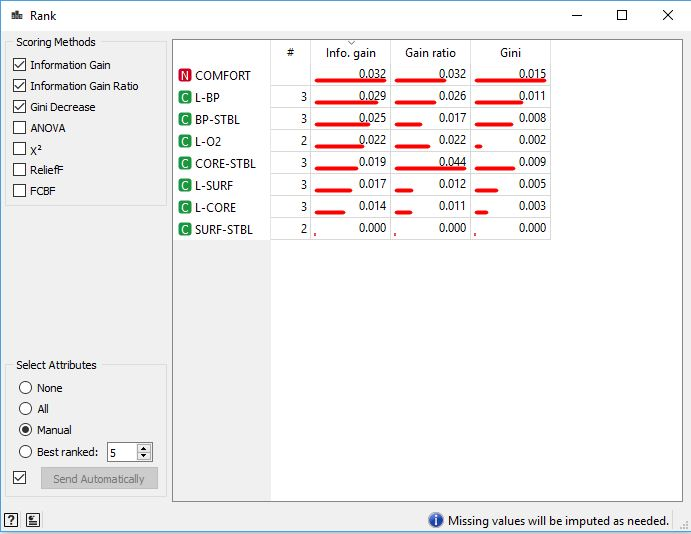
\includegraphics[scale = 0.5]{img/rank.JPG}
	\caption{informazione di ogni attributo }\label{fig:1}
\end{figure}
\begin{figure}
	\centering
	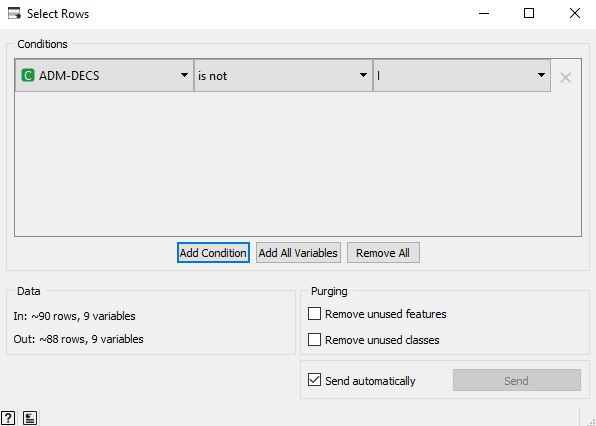
\includegraphics[scale = 0.4]{img/rows.JPG}
	\caption{selezione dei record non di classe I}	\label{fig:2}
\end{figure}	
\section{Trattamento dati mancanti}
Nel Db sono presenti solo 3 dati mancanti nell'attributo comfort. Dato che sono pochi, ho più dati di quelli richiesti dalla regola del pollice e poiché l'attributo ha molta informazione, preferisco eliminare le istanze, in modo da non influenzare la classificazione con dei valori medi non necessariamente corretti.
Pertanto utilizzo in Orange la widget \emph{'impute'} e seleziono \emph{'rimuovi istanze con valori sconosciuti'}, come riportato in figura \ref{fig:3}.
\begin{figure}	
	\centering
	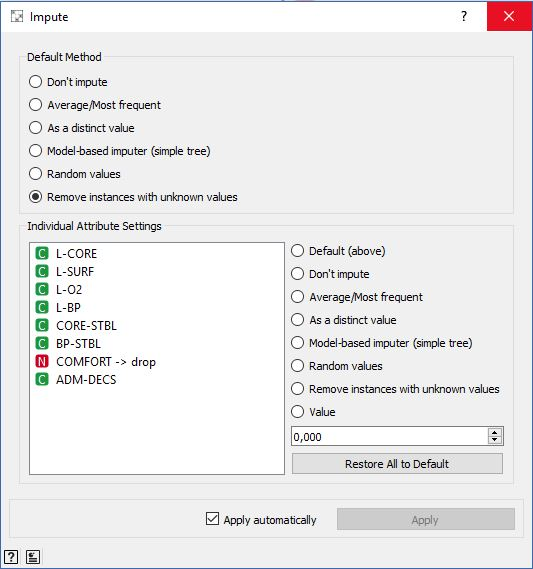
\includegraphics[scale = 0.45]{img/imputing.JPG}
	\caption{imputing dei dati mancanti }\label{fig:3}
\end{figure}
\section{Discretizzazione}
Prima di procedere, noto dai box-plot che l'attributo COMFORT è un numero tra 0 e 20 ma che si concentra intorno al 10, inoltre vedendo la distribuzione molto precisa, si vedono due picchi in 10 e 15 e guardando la tabella dei dati vedo come in realtà siano utilizzati solo quattro valori: 5, 7, 10 e 15 . Decido di discretizzare COMFORT in tre valori: basso, medio, alto con soglie poste a 8.5 e 12.5.


\section{Correlazione}
Infine cerco eventuali correlazioni per ridurre ulteriormente gli attributi, infatti se due o più attributi sono fortemente correlati non è necessario disporre di entrambi per arrivare alla medesima conclusione. Inoltre l'indipendenza fra gli attributi è un assunzione di alcuni modelli tra cui il Naive Bayes che confronteremo. Ciò che mi aspetto è una correlazione tra la temperatura interna ed esterna. Utilizzo la widget scatter-plot per avere una visualizzazione grafica delle relazioni fra gli attributi due a due. A un primo sguardo non c'è nessuna correlazione fra gli attributi, neanche quella che mi aspettavo. La conferma dell'assenza di correlazioni è data anche dalla widget 'Sieve Diagrams'.  

Infatti, un 'Sieve Diagrams' è un metodo grafico per visualizzare le frequenze in una tabella di contingenza a due vie in relazione alle frequenze aspettate sotto l'assunzione di indipendenza e sottolinea possibili pattern fra due attributi. Dunque l’area di ogni rettangolo è proporzionale alla frequenza attesa,  mentre la frequenza osservata si vede dal numero di quadrati in ogni rettangolo. L'intensità del colore evidenzia una deviazione dall'indipendenza, in rosso positiva, in blu negativa. Nel nostro caso i colori sono appena accennati, quindi gli attributi possono essere considerati indipendenti.
\begin{figure}	
	\centering
	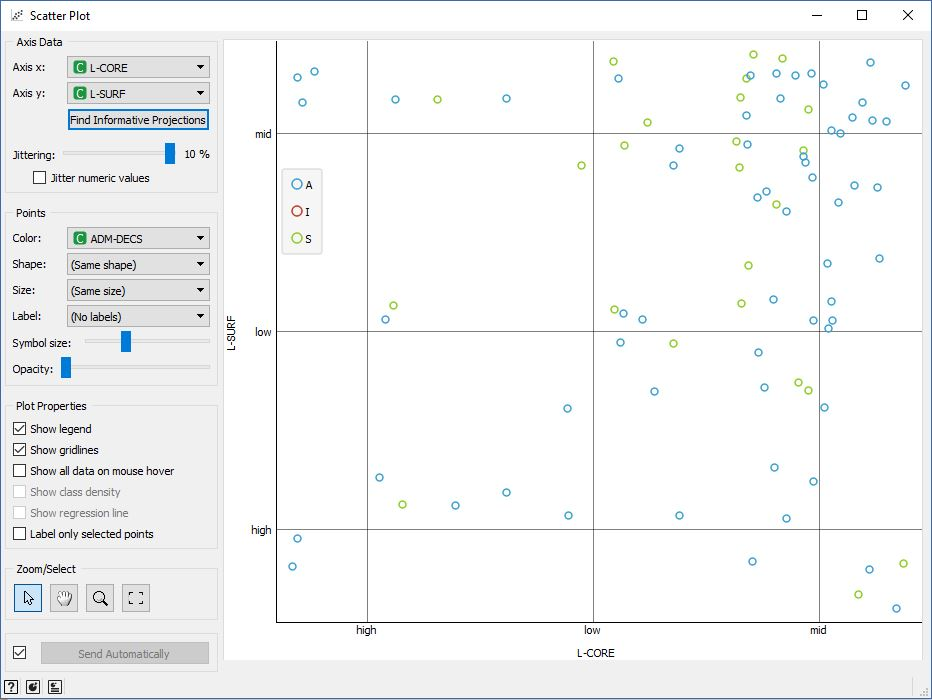
\includegraphics[scale = 0.5]{img/ScatterJPG.JPG}
	\caption{Scatter plot che non evidenzia correlazioni tra temperatura esterna e interna }\label{fig:4}
\end{figure}
\begin{figure}	
	\centering
	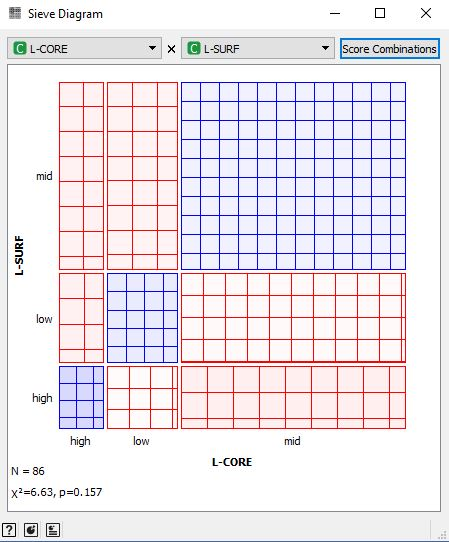
\includegraphics[scale = 0.6]{img/Sieve.JPG}
	\caption{Diagramma di Sieve che non evidenzia correlazioni tra temperatura esterna e interna }\label{fig:5}
\end{figure}
\chapter{Confronto tra classificatori}
Dopo il pre-processing dei dati, vogliamo ora trovare un buon classificatore per decidere se il paziente deve essere assegnato a un piano o dimesso. Il nostro primo riferimento sarà il classificatore di maggioranza. Sarà difficile batterlo perché il database è molto rumoroso e la percentuale di pazienti da affidare a un piano è molto superiore alla percentuale dei dimessi.
Andremo ad analizzare i seguenti classificatori:
\begin{itemize}
	\item Albero decisionale,
	\item Naive Bayes,
	\item Logistic regression,
	\item K-Nearest-Neighbours,
	\item CN2 rule induction.
\end{itemize}		
	Prima di ispezionare i classificatori, però, dividiamo i dati per effettuare il training e i test. Divido i dati con la widget 'Data Sampler' con sampling type proporzione fissa al 30\% stratificato. 
	
	Dunque i dati generati verranno utilizzati per fare i test finali per mantenere l'indipendenza, mentre divido ulteriormente le istanze rimanenti (70\%) con sampling type 'cross validation' con 5 fold e opzioni dati stratificati e replicabili. Dunque farò il training 5 volte usando ogni volta a rotazione 4 fold per i training e 1 per i test e analizzerò gli indici di accuratezza e AUC per fare i confronti.
	
	\section{I Classificatori}
		\subsection{L'Albero Decisionale}
		L'albero decisionale è anche detto classificatore universale, è un modello ad alta varianza adatto quando si hanno attributi discreti e tanti dati. Il suo punto forte è la capacità di classificare dati con superfici di separazione non lineari. Avendo alta varianza, perché funzioni bene è necessario utilizzare tecniche di pruning per evitare una perfetta accuratezza di ricostituzione, ma una scarsa accuratezza di generalizzazione. Quindi impostiamo alcuni parametri di forward pruning come si può vedere in figura \ref{fig:6}.
\begin{figure}	
	\centering
	\includegraphics[scale = 0.8]{img/Tree.JPG}
	\caption{Parametri del modello 'Albero Decisionale' utilizzato. }\label{fig:6}
\end{figure}
	\subsection{Naive Bayes}
	Il classificatore Naive Bayes è un semplice modello probabilistico, basato sulla forte assunzione di indipendenza degli attributi. 
	
	Il suo modello è: 
	\begin{equation}
	P(C|X) = \frac{P(C)*P(X|C)}{P(X)}
	\end{equation}
	\begin{itemize}
		\item P(C) = probabilità della classe,
		\item P(X) = probabilità degli attributi
	\end{itemize}
	Essendoci l'assunzione di indipendenza possiamo scrivere:
	\begin{equation}
	C = argmax (P(C)*\prod_{}{}{P(X|C)})
	\end{equation}
	Nel nostro database gli attributi sembrano effettivamente indipendenti e grazie alla feature selection abbiamo solo i più informativi, quindi il Naive Bayes potrebbe essere un buon classificatore per il nostro database.
	\subsection{Logistic Regression}
	La regressione logistica è un modello discriminativo, cioè che stima direttamente la probabilità a posteriori della classe, dati gli attributi. E' in grado di modellizzare le relazioni fra gli attributi sia continui, sia categorici, sia binari e una classe binaria come nel nostro caso (è tuttavia possibile estenderla a casi con più classi). L'utilizzo della funzione logistica e della logit permette di avere una semplice trasformazione di P(C|X) e una relazione lineare con gli attributi. Per decidere la classe viene utilizzata la stima a massima verosomiglianza.

	\subsection{K-Nearest-Neighbours}
	Il K-Nearest-Neighbours è il classificatore più semplice in termini di implementazione e logica, è un classificatore \emph{pigro}, che bada solo a una funzione di distanza per scegliere. Funziona bene con attributi continui. 
	
	Nel caso di attributi categorici, come nel nostro database, si considera una distanza pari a 0 in caso di valori uguali e un numero (solitamente 1) in caso di valori diversi. Dal momento che i nostri attributi sono categorici e spesso a più valori, è probabile che questo classificatore non sia il più performante, tuttavia verrà confrontato.
	
	
Il KNN non fa altro che guardare a quale classe sono assegnati i k esempi più vicini al nuovo caso e lo assegna alla classe di maggioranza. 

Più k è grande più si evita il rumore, ma si rende più labile la classificazione, di solito si sceglie k>=3. 

Dunque i parametri del classificatore sono un numero intero k e una funzione di distanza. Ho scelto di utilizzare k = 5 e la distanza euclidea come mostrato in figura \ref{fig:7}.
\begin{figure}	
	\centering
	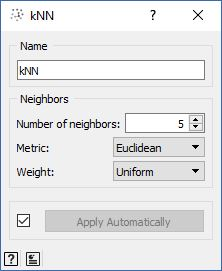
\includegraphics[scale = 0.8]{img/Knn.JPG}
	\caption{Parametri del modello 'K-Nearest-Neighbours' utilizzato.}\label{fig:7}
\end{figure}	
\subsection{CN2 Rule Induction}
E' un algoritmo di covering diretto che, dunque, estrae regole dai dati. Per trovare una nuova regola viene effettuata una ricerca a fascio dove si continua a tener conto di varie possibili regole candidate chiamate complessi, l'insieme di queste si chiama stella.
Viene utilizzata una statistica di verosomiglianza per valutare la significatività di ogni complesso e quindi decidere quale regola decisionale scegliere. 

Nel nostro caso con attributi categorici può essere una buona soluzione.
	
\section{Confronto finale tra classificatori e scelta del migliore}
Ora che abbiamo visto in breve le caratteristiche di ogni classificatore testato, passiamo a guardare i risultati ottenuti. 

Con il 70\% dei dati presi in modo stratificato, ho utilizzato la widget rank per utilizzare solo gli attributi più informativi, e poi ancora la widget data sampler con 5-fold-cross-validation utilizzando 4 fold come training e uno come test set.

Infine ho dato in input alla widget 'test and score ' i dati di training, di test e i classificatori discussi e ho salvato i report dei cinque test. 


Per valutare le performance di ogni classificatore andremo a valutare alcuni indici quali:
\begin{itemize}
\item l'Accuratezza: percentuale dei casi classificati correttamente,
\item l'AUC: l'area sotto la curva di ROC la quale grafica le performance del classificatore al variare della soglia decisionale, 
\item la Precision:  percentuale di istanze effettivamente positive tra quelle classificate come tali,
\item la Recall: rappresenta la percentuale di casi positivi classificati come tali,
\item indice F: media armonica tra recall e precision.
\end{itemize}
Dopo dei primi test, ho scelto nella widget rank di utilizzare i tre attributi con rank più alto, infatti testando con solo due, o più di quattro, si trovavano un' AUC e un'accuratezza generalmente peggiori. E' importante selezionare bene gli attributi, perché troppi attributi poco informativi confondono solo la classificazione, migliorando l'accuratezza di ricostituzione, ma peggiorando quella più interessante di generalizzazione.

Con Matlab, dunque,  ho calcolato le medie delle accuratezze e grazie alla t di student gli intervalli di confidenza di ogni classificatore che riporto in tabella \ref{tab:1}.
\begin{table}
\centering
\caption{Tabella con accuratezze medie.}
\label{tab:1}
\begin{tabular}{|l|c|c|c|l|}
\hline
Classificatore & Accuratezza media & CI inf  & CI sup\\
\hline
KNN & 0.5278 & 0,3165 & 0,7391\\
\hline
Regressione Logistica & 0.6686 & 0,5645 & 0,7738\\
\hline
Albero Decisionale & 0.6688 & 0,5119 & 0,8257\\
\hline
CN2 & 0.6840 & 0,5645 & 0,8035\\
\hline
Naive Bayes & 0.6994 & 0,6131 & 0,7857\\
\hline
Maggioranza & 0.7176 & 0,6863 & 0,7489\\
\hline

\end{tabular}
\end{table}

Come si può vedere, in media, il classificatore di maggioranza resta il migliore.

E' un risultato che mi aspettavo, dal momento che il dataset è molto rumoroso e sbilanciato. 

Subito dopo trovo il classificatore Naive Bayes e il CN2: i loro intervalli di confidenza sono più larghi e sono simili a quelli della regressione logistica che tuttavia ha un'accuratezza media più bassa.

 Il KNN è il peggiore: mi aspettavo che non andasse molto bene, perché è un classificatore basato sulle distanze e quindi opera meglio con attributi continui rispetto ai discreti a più valori.

Tuttavia oltre all'accuratezza, analizzo anche l'AUC, infatti il classificatore di maggioranza, sceglie sempre la classe più frequente, nel nostro caso la A, a noi invece interessa un classificatore che sia in grado di stabilire anche la S. 

L'AUC del classificatore di maggioranza è 0.5 per definizione, cioè è come se il modello andasse a caso, la sua scelta dipende dalla soglia ottima della curva di ROC, scegliendo la sensitività a 1.

\noindent Quindi analizzo il comportamento degli altri classificatori.

Tutti i classificatori tranne l'albero decisionale hanno un' AUC maggiore di 0.5, l'ottimale sarebbe che fosse vicino a 1. 

In questo caso il classificatore migliore si rivela essere il Naive Bayes, seguito dalla regressione logistica.

Per decidere allora il miglior classificatore, utilizzo un'altra widget 'test and score' con come test set il 30\% del primo data sampler in modo da assicurarmi l'indipendenza dal training set utilizzato prima, come training set i dati ridotti e come classificatori da valutare il Naive Bayes, la regressione logistica e il CN2.

Riporto in figura \ref{fig:8} i risultati . 

Finalmente ho scelto come classificatore migliore il Naive Bayes, in quanto sia in accuratezza, in AUC e in Precision ha risultati lievemente migliori degli altri. Anche guardando la matrice di confusione è l'unico che riesce ad individuare casi di dimissione e, quindi, ad avere meno falsi positivi.

\begin{table}
\centering
\caption{Tabella con AUC medie.}
\label{tab:2}
\begin{tabular}{|l|c|c|c|l|}
\hline
Classificatore & AUC media\\
\hline
Albero Decisionale & 0.4838\\
\hline
Maggioranza & 0.500\\
\hline
KNN & 0.5204\\
\hline
CN2 & 0.5468\\
\hline
Regressione Logistica & 0.5962 \\
\hline
Naive Bayes & 0.6950 \\
\hline
\end{tabular}
\end{table}
\begin{figure}	
	\centering
	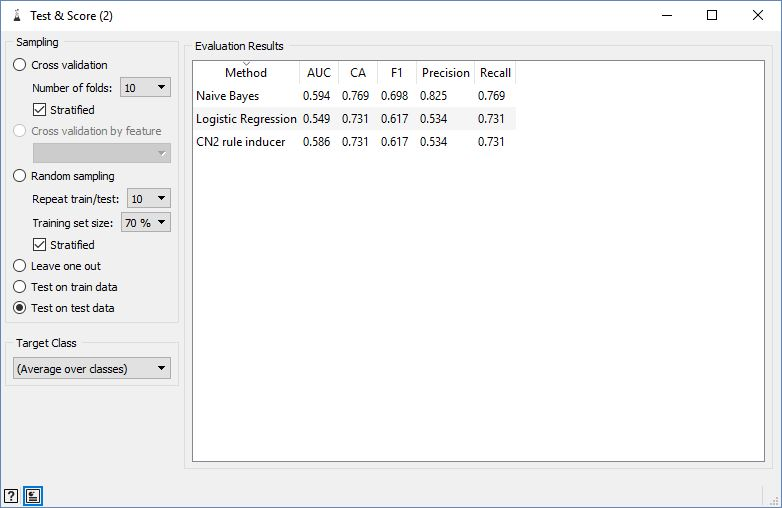
\includegraphics[scale = 0.5]{img/score.JPG}
	\caption{Risultati test sul test set indipendente.}\label{fig:8}
\end{figure}
\begin{figure}	
	\centering
	\includegraphics[scale = 0.6]{img/ROC.JPG}
	\caption{Curva di ROC dei tre classificatori migliori.}\label{fig:9}
\end{figure}

\appendix
\chapter{Codice Matlab}
\begin{lstlisting}[
style=Matlab-editor,
basicstyle=\mlttfamily
]
clc
close all
clear all

\% accuratezze trovate con la 5-fold cross validation
acc_albero = [0.769 0.462 0.750 0.727 0.636];
acc_constant = [0.692 0.692 0.750 0.727 0.727];
acc_log = [0.692 0.538 0.750 0.727 0.636];
acc_naive = [0.769 0.615 0.750 0.727 0.636];
acc_knn = [0.692 0.462 0.667 0.273 0.545];
acc_cn2 = [0.769 0.538 0.750 0.727 0.636];

\% accuratezze medie
mean_acc_albero = mean(acc_albero);
mean_acc_constant = mean(acc_constant);
mean_acc_log = mean(acc_log);
mean_acc_naive = mean(acc_naive);
mean_acc_knn = mean(acc_knn);
mean_acc_cn2 = mean(acc_cn2);

accuratezza = [acc_albero' acc_constant' acc_log' acc_naive' acc_knn' acc_cn2'];
[p_acc, table_acc, stats_acc] = anova2(accuratezza,1)
c_acc = multcompare(stats_acc)
\% intervalli di confidenza
CI_Albero = InterConf(acc_albero);
CI_constant = InterConf(acc_constant);
CI_log = InterConf(acc_log);
CI_naive = InterConf(acc_naive);
CI_knn = InterConf(acc_knn);
CI_cn2 = InterConf(acc_cn2);

\%auc 
AUC_albero = [0.583 0.431 0.593 0.312 0.500]; 
AUC_constant = [0.5 0.5 0.5 0.5 0.5];
AUC_log = [0.694 0.472 0.815 0.500 0.500];
AUC_naive = [0.639 0.583 0.815 0.938 0.500];
AUC_knn = [0.556 0.514 	0.741 0.312 0.479];
AUC_cn2 = [0.583 0.653 0.685 0.188 0.625];

\%AUC medie
mean_AUC_albero = mean(AUC_albero);
mean_AUC_constant = mean(AUC_constant);
mean_AUC_log = mean(AUC_log);
mean_AUC_naive = mean(AUC_naive);
mean_AUC_knn = mean(AUC_knn);
mean_AUC_cn2 = mean(AUC_cn2);

auc = [AUC_albero' AUC_constant' AUC_log' AUC_naive' AUC_knn' AUC_cn2'];
[p_AUC, table_AUC, stats_AUC] = anova2(auc,1)
c_AUC = multcompare(stats_AUC)
\end{lstlisting}

\begin{lstlisting}[
style=Matlab-editor,
basicstyle=\mlttfamily
]
function [ CI ] = InterConf( x )

SEM = std(x)/sqrt(length(x));
ts = tinv([0.025  0.975],length(x)-1);
CI = mean(x) + ts*SEM ;

end
\end{lstlisting}
\chapter{Script Orange}
	\centering
	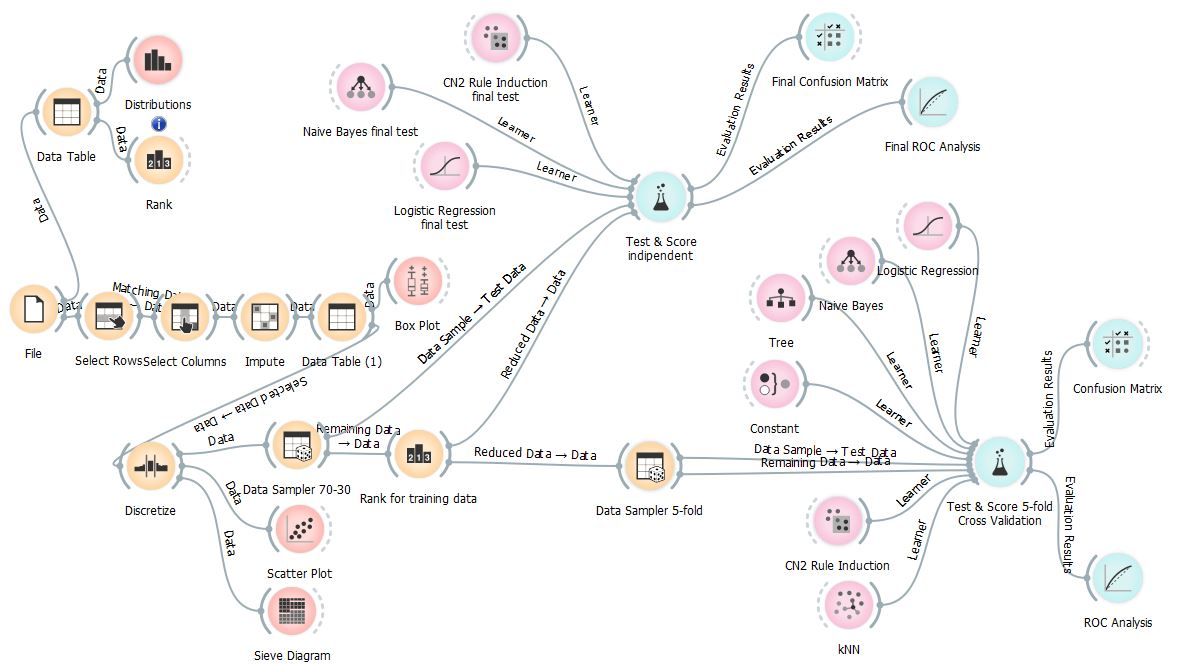
\includegraphics[scale = 0.5]{img/Orange.JPG}
\end{document}
